\documentclass[12pt,onecolumn]{article}
\usepackage[utf8]{inputenc} % UTF8 input encoding
\usepackage[T2A]{fontenc}   % T2A font encoding for Cyrillic script
\usepackage[russian]{babel} % Russian language support
\usepackage{listings}
\usepackage{float}
\usepackage{mathtools}
\usepackage{longtable}
\everymath{\displaystyle}
\usepackage{listings} 
\usepackage[usenames]{color}
\usepackage[html]{xcolor}
\usepackage{framed}
\usepackage{csquotes}
\usepackage{geometry}

\geometry{
  a4paper,
  top=25mm, 
  right=5mm, 
  bottom=25mm, 
  left=5mm
}

\begin{document}
\setcounter{tocdepth}{4}
\begin{center}
    Федеральное государственное автономное образовательное учреждение высшего образования "Национальный Исследовательский Университет ИТМО"\\ 
    Мегафакультет Компьютерных Технологий и Управления\\
    Факультет Программной Инженерии и Компьютерной Техники \\
    
\includegraphics[scale=0.3]{image/itmo.jpg} % нужно закинуть картинку логтипа в папку с отчетом
\end{center}
\vspace{1cm}


\begin{center}
    \textbf{Лабораторная работа №1}\\
    по дисциплине\\
    \textbf{'Архитектура программных систем'}\\
\end{center}

\vspace{2cm}

\begin{flushright}
  Выполнил Студент  группы P33102\\
  \textbf{Лапин Алексей Александрович}\\
  Преподаватель: \\
  \textbf{Перл Иван Андреевич}\\
\end{flushright}

\vspace{6cm}
\begin{center}
    г. Санкт-Петербург\\
    2023г.
\end{center}

\newpage
\tableofcontents
\newpage

\section{Текст задания}
Выбрать любую реально существующую систему и описать её в терминах UML. Желательно, чтобы система была не полностью информационной, но опиралась на информационную систему как показано в примере на лекции (Point of sale). Необходимо описать границы системы на разных уровнях, а также описать сценарии использования для нескольких Акторов.\\
\textbf{Отчёт по работе должен содержать:}
\begin{enumerate}
  \item Титульный лист с указанием автора и номера группы
  \item Само задание
  \item Описание рассматриваемой системы с требованиями к ней
  \item Формальное описание системы с необходимым количеством UML диаграмм
  \item Словесное описание сценариев сценариев использование для рассматриваемых акторов
\end{enumerate}
\section{Описание рассматриваемой системы с требованиями к ней}
Онлайн магазин для тренеров (= пользователь) по продаже покемонов и камней эволюции.\\
Возможности:
\begin{itemize}
  \item Ввести свои характеристи (стиль игры, уровень, своих покемонов) и получить рекомендованные к покупке покемоны
  \item Положить понравившихся покемонов в корзину
  \item Оформить заказ
  \item Отслеживать статус заказа
  \item Посмотреть покупки
\end{itemize}
\subsection{Функциональные требования (FR)}
\textbf{Требования администратора сайта:}
\begin{enumerate}
  \item Возможность добавить товар в каталог
  \item Возможность удалять товар из каталога
  \item Возможность изменять характеристики товара в каталоге
  \item Возможность видеть заказы всех пользователей
  \item Возможность изменять статус заказа
\end{enumerate}
\textbf{Требования пользователя:}
\begin{enumerate}
  \item Возможность регистрации
  \item Возможность авторизации
  \item Возможность просмотра каталога
  \item Возможность просмотра информации о выбранном товаре
  \item Возможность добавления товара в корзину
  \item Возможность оформления заказа из корзины
  \item Возможность отслеживания статуса заказа
  \item Возможность получить рекомендованные к покупке покемоны
  \item Возможность редактирования профиля
\end{enumerate}
\subsection{Нефункциональные требования (NR)}
\begin{enumerate}
  \item Сайт должен корректно работать во всех современных браузерах. Такие как:
  Google Chrome, Mozilla Firefox, Microsoft Edge, Яндекс.Браузер.
  \item Сайт должен быть адаптирован под мобильные устройства.
  \item Backend должен быть написан на языке программирования Java с фреймворком Java Spring.
  \item Frontend должен быть написан на языке программирования JavaScript с использованием библиотеки React.
  \item Хранение данных должно быть реализовано с помощью СУБД PostgreSQL.
  \item Сайт должен быть развернут на helios
  \item Сайт должен быть защищён от SQL инъекций
\end{enumerate}
\section{Формальное описание системы с необходимым количеством UML диаграмм}
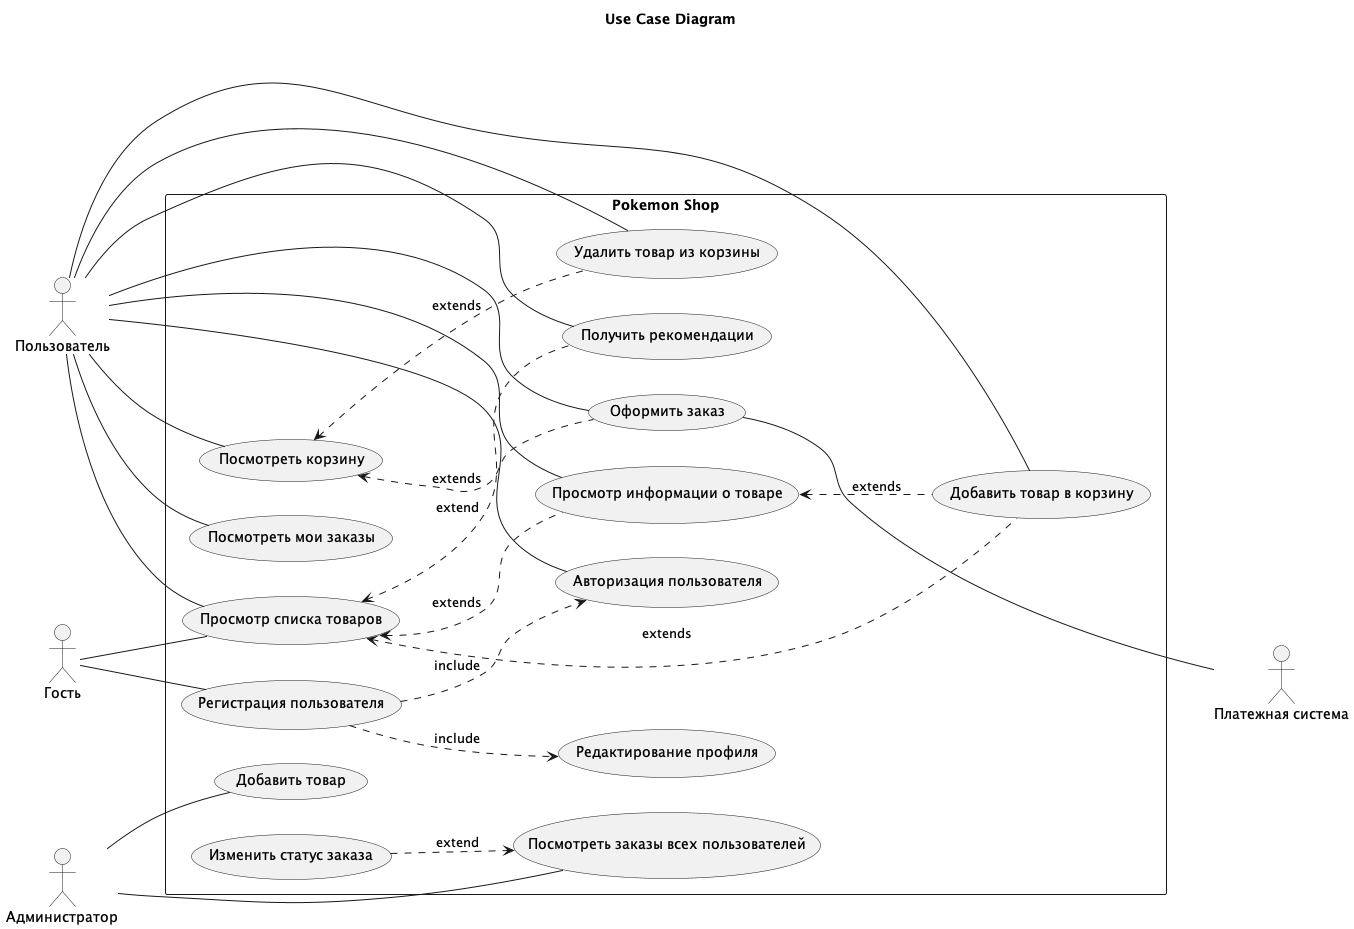
\includegraphics[width=\textwidth]{image/usecase.png}\\
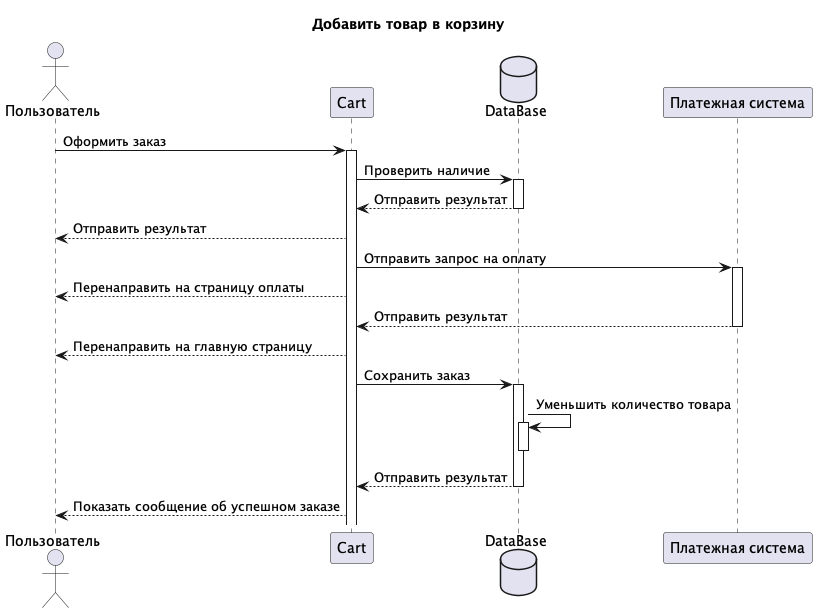
\includegraphics[width=0.7\textwidth]{image/sequence.png}\\
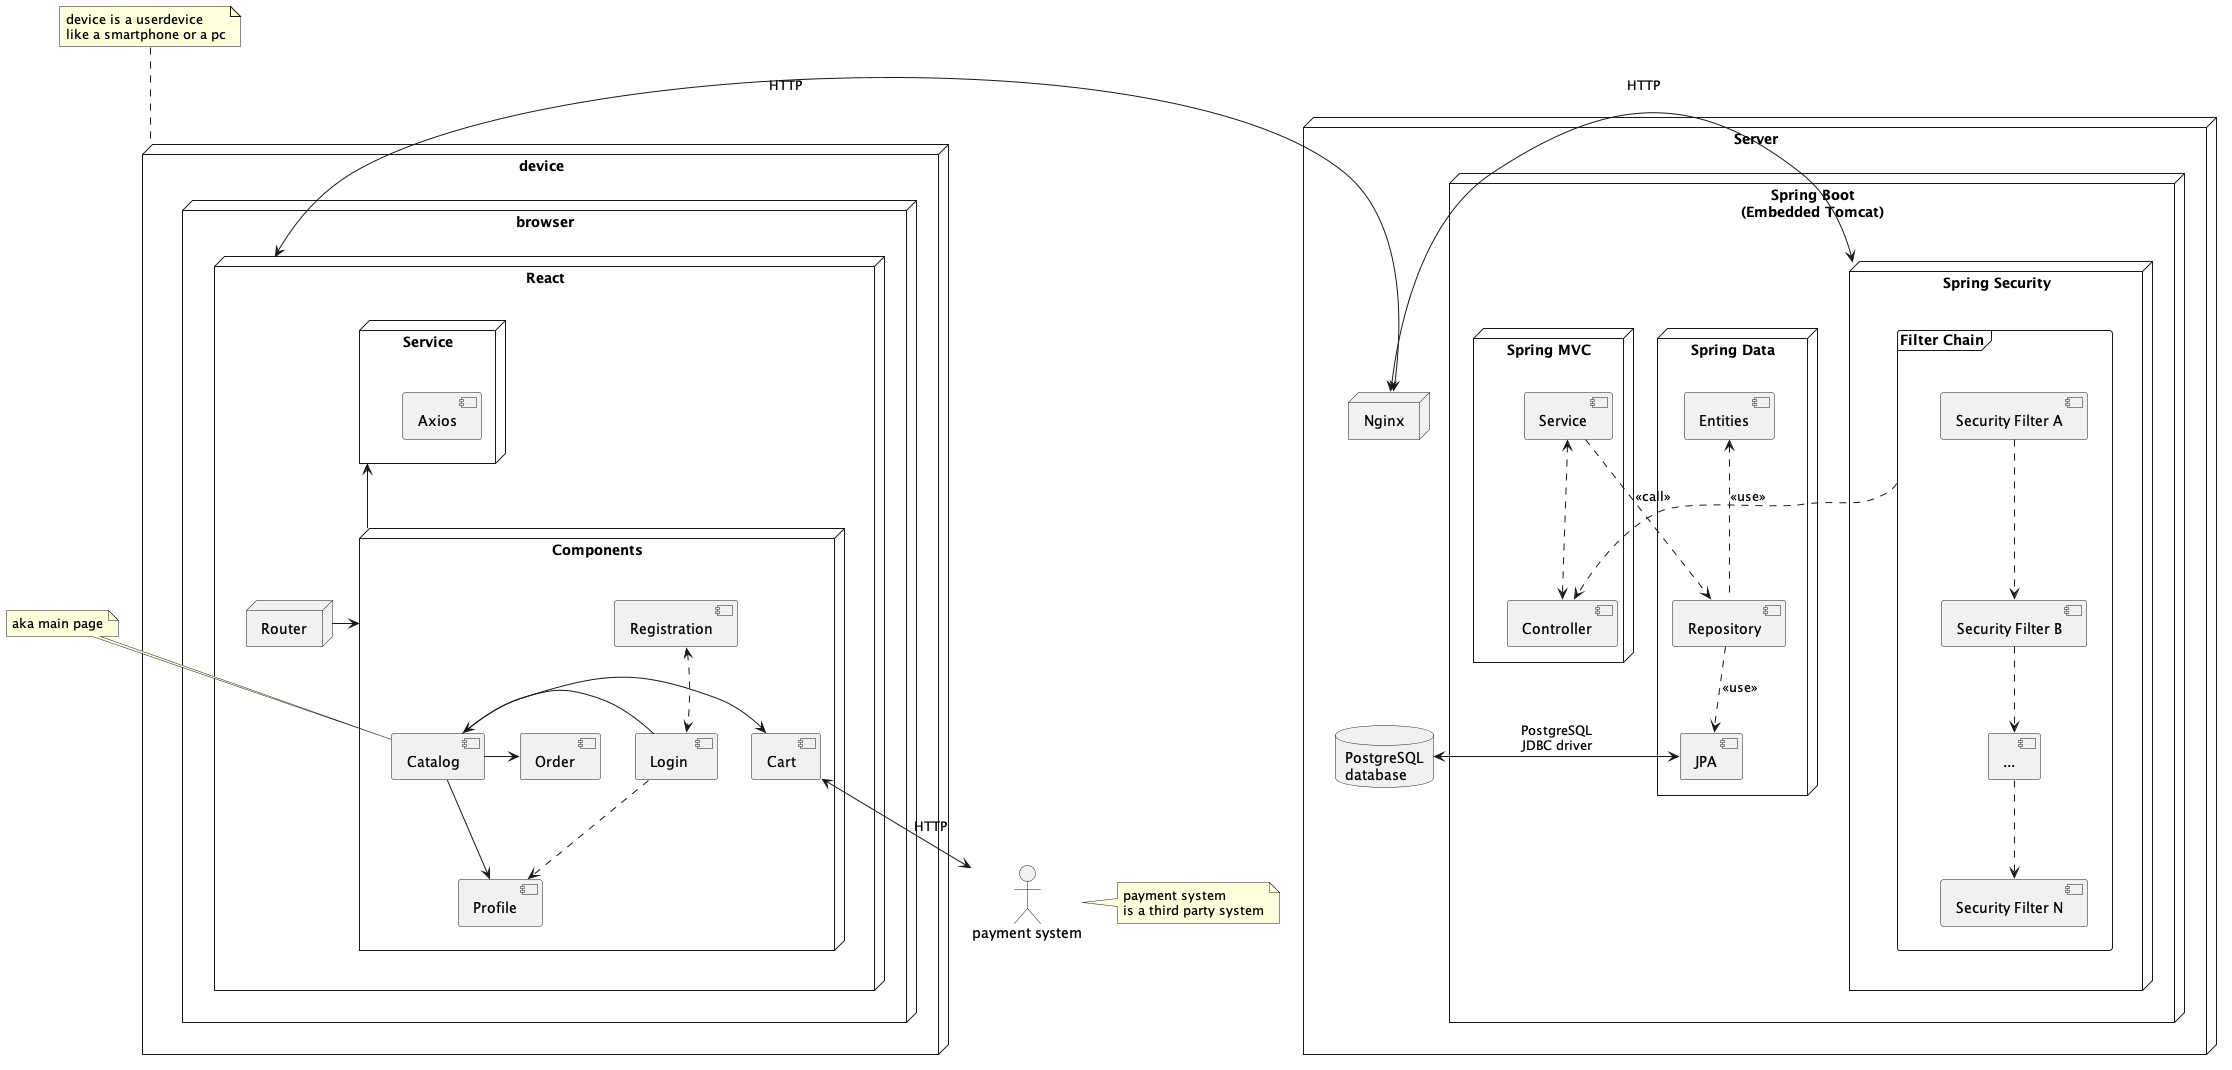
\includegraphics[width=\textwidth]{../out/Lab1/component/component_diagram.png}\\

\section{Словесное описание сценариев сценариев использование для рассматриваемых акторов}
\begin{longtable}{|l|l|}
  \hline
  Название сценария & Регистрация                                             \\ \hline
  \endfirsthead
  %
  \endhead
  %
  Краткое описание  & Гость хочет создать свой личный кабинет на сайте \\ \hline
  Акторы            & Гость                                            \\ \hline
  Предусловия       & Гость не зарегистрирован на сайте                \\ \hline
  Основной поток &
    \begin{tabular}[c]{@{}l@{}}1. Гость нажимает на кнопку "Sign up"\\2. Система отображает форму регистрации\\ 3. Гость вводит свои данные\\ 4. Пользователь нажимает на кнопку "Sign up"\\ 5. Система регистрирует пользователя\\ 6. Система перенаправляет пользователя на главную страницу\\ 7. Система отображает сообщение об успешной регистрации\end{tabular} \\ \hline
  Постусловия       & Пользователь может войти в свой личный кабинет          \\ \hline
\end{longtable}
\begin{longtable}{|l|l|}
  \hline
  Название сценария & Авторизация                                             \\ \hline
  \endfirsthead
  %
  \endhead
  %
  Краткое описание  & Пользователь хочет войти в свой личный кабинет \\ \hline
  Акторы            & Пользователь                                            \\ \hline
  Предусловия       & Пользователь зарегистрирован на сайте                \\ \hline
  Основной поток &
    \begin{tabular}[c]{@{}l@{}}1. Пользователь нажимает на кнопку "Sign in"\\2. Система отображает форму авторизации\\ 3. Пользователь вводит свои данные\\ 4. Пользователь нажимает на кнопку "Sign in"\\ 5. Система авторизирует пользователя\\ 6. Система перенаправляет пользователя на главную страницу\\ 7. Система отображает сообщение об успешной авторизации\end{tabular} \\ \hline
  Постусловия       & Пользователь может войти в свой личный кабинет          \\ \hline
\end{longtable}
\begin{longtable}{|l|l|}
  \hline
  Название сценария & Просмотр списка товаров \\ \hline
  \endfirsthead
  %
  \endhead
  %
  Краткое описание  & Пользователь хочет посмотреть список товаров \\ \hline
  Акторы            & Пользователь                                            \\ \hline
  Предусловия       & Пользователь зарегистрирован на сайте                \\ \hline
  Основной поток &
    \begin{tabular}[c]{@{}l@{}}1. Пользователь переходит на главный \\2. Система отображает каталог товаров разделенные на две секции:\\ "Покемоны" и "Камни"\\ 3. Пользователь видит карточки товаров, на которых содержится preview товара,\\ его название и цена, а также кнопка "Add to cart"\end{tabular} \\ \hline
  Постусловия       &    -       \\ \hline
\end{longtable}
\begin{longtable}{|l|l|}
  \hline
  Название сценария & Просмотр информации о товаре  \\ \hline
  \endfirsthead
  %
  \endhead
  %
  Краткое описание  & Пользователь хочет посмотреть информацию о товаре \\ \hline
  Акторы            & Пользователь                                            \\ \hline
  Предусловия       & Пользователь зарегистрирован на сайте                \\ \hline
  Основной поток & 
  \begin{tabular}[c]{@{}l@{}}
    1. Пользователь нажимает на карточку товара в каталоге\\
    2. Система отображает страницу с информацией о товаре\\
    3. Пользователь видит название товара, его цену, описание,\\
    а также кнопку "Add to cart"
  \end{tabular} \\ \hline
  Постусловия       &    -       \\ \hline
\end{longtable}
\begin{longtable}{|l|l|}
  \hline
  Название сценария & Добавление товара в корзину  \\ \hline
  \endfirsthead
  %
  \endhead
  %
  Краткое описание  & Пользователь хочет добавить товар в корзину \\ \hline
  Акторы            & Пользователь                                            \\ \hline
  Предусловия       & Пользователь зарегистрирован на сайте                \\ \hline
  Основной поток &
    \begin{tabular}[c]{@{}l@{}}1. Пользователь нажимает на кнопку "Add to cart"\\2. Система добавляет товар в корзину\\ 3. Система отображает сообщение об успешном добавлении товара в корзину\end{tabular} \\ \hline
  Постусловия       & Состояние корзины сохраняется в куки пользователя        \\ \hline
\end{longtable}
\begin{longtable}{|l|l|}
  \hline
  Название сценария & Просмотреть корзину  \\ \hline
  \endfirsthead
  %
  \endhead
  %
  Краткое описание  & Пользователь хочет посмотреть товары в корзине \\ \hline
  Акторы            & Пользователь                                            \\ \hline
  Предусловия       & Пользователь авторизован на сайте                \\ \hline
  Основной поток &
    \begin{tabular}[c]{@{}l@{}}1. Пользователь нажимает на кнопку "Cart"\\2. Система отображает страницу с корзиной\\ 3. Система отображает список товаров в корзине, а также их количество и цену\end{tabular} \\ \hline
  Постусловия       & -      \\ \hline
\end{longtable}
\begin{longtable}{|l|l|}
  \hline
  Название сценария & Удалить товар из корзины \\ \hline
  \endfirsthead
  %
  \endhead
  %
  Краткое описание  & Пользователь хочет удалить товар из корзины \\ \hline
  Акторы            & Пользователь                                            \\ \hline
  Предусловия       & Пользователь авторизован на сайте                \\ \hline
  Основной поток &
    \begin{tabular}[c]{@{}l@{}}1. Пользователь нажимает на кнопку "Delete"\\2. Система удаляет товар из корзины\\ 3. Система отображает сообщение об успешном удалении товара из корзины\end{tabular} \\ \hline
  Постусловия       & Новое состояние корзины сохраняется в куки пользователя        \\ \hline
\end{longtable}

\begin{longtable}{|l|l|}
  \hline
  Название сценария & Оформление заказа  \\ \hline
  \endfirsthead
  %
  \endhead
  %
  Краткое описание  & Пользователь хочет оформить заказ \\ \hline
  Акторы            & Пользователь                                            \\ \hline
  Предусловия       & Пользователь авторизован на сайте                \\ \hline
  Основной поток &
    \begin{tabular}[c]{@{}l@{}}1. Пользователь нажимает на кнопку "Checkout"\\2. Система отображает страницу с оформлением заказа\\ 3. Пользователь вводит свои данные\\ 4. Пользователь нажимает на кнопку "Checkout"\\ 5. Система перенаправляет на страницу оплаты сторонней платежной системы и сохраняет заказ в базе данных\\ 6. Система принимает ответ от сторонней платежной системы \\7. Система перенаправляет пользователя на главную страницу\\ 8. Система отображает сообщение об успешном оформлении заказа\end{tabular} \\ \hline
    Постусловия       & Заказ сохранен в базе данных со статусом     \\ \hline
  \end{longtable}
\begin{longtable}{|l|l|}
    \hline
    Название сценария & Посмотреть статус заказа  \\ \hline
    \endfirsthead
    %
    \endhead
    %
    Краткое описание  & Пользователь хочет посмотреть статус заказа \\ \hline
    Акторы            & Пользователь                                            \\ \hline
    Предусловия       & Пользователь авторизован на сайте                \\ \hline
    Основной поток &
      \begin{tabular}[c]{@{}l@{}}1. Пользователь нажимает на кнопку "Orders"\\2. Система отображает страницу с заказами\\ 3. Пользователь видит список своих заказов, а также их статусы\end{tabular} \\ \hline
      Постусловия       & -     \\ \hline
  \end{longtable}
  \begin{longtable}{|l|l|}
    \hline
    Название сценария & Получить рекомендации  \\ \hline
    \endfirsthead
    %
    \endhead
    %
    Краткое описание  & Пользователь хочет рекомендованные к покупке покемоны \\ \hline
    Акторы            & Пользователь                                            \\ \hline
    Предусловия       & Пользователь заполнил свои характеристики в профиле               \\ \hline
    Основной поток &
      \begin{tabular}[c]{@{}l@{}}1. Пользователь нажимает на кнопку "Recommendations"\\2. Система отображает страницу с рекомендациями\\ 3. Система отображает список рекомендованных к покупке покемонов\end{tabular} \\ \hline
      Постусловия       & -     \\ \hline
  \end{longtable}
  \begin{longtable}{|l|l|}
    \hline
    Название сценария & Редактировать профиль  \\ \hline
    \endfirsthead
    %
    \endhead
    %
    Краткое описание  & Пользователь хочет редактировать свой профиль \\ \hline
    Акторы            & Пользователь                                            \\ \hline
    Предусловия       & Пользователь авторизован на сайте                \\ \hline
    Основной поток &
      \begin{tabular}[c]{@{}l@{}}1. Пользователь нажимает на кнопку "Profile"\\2. Система отображает страницу с профилем\\ 3. Пользователь нажимает на кнопку "Edit"\\ 4. Система отображает форму редактирования профиля\\ 5. Пользователь вводит свои данные\\ 6. Пользователь нажимает на кнопку "Save"\\ 7. Система сохраняет изменения в базе данных\\ 8. Система перенаправляет пользователя на страницу профиля\\ 9. Система отображает сообщение об успешном редактировании профиля\end{tabular} \\ \hline
      Постусловия       & Изменения сохранены в базе данных     \\ \hline
  \end{longtable}
  \begin{longtable}{|l|l|}
    \hline
    Название сценария & Добавить товар \\ \hline
    \endfirsthead
    %
    \endhead
    %
    Краткое описание  & Администратор сайта хочет добавить товар в каталог \\ \hline
    Акторы            & Администратор                                            \\ \hline
    Предусловия       & Администратор авторизован на сайте                \\ \hline
    Основной поток &
      \begin{tabular}[c]{@{}l@{}}1. Администратор нажимает на кнопку "Add product"\\2. Система отображает форму добавления товара\\ 3. Администратор вводит данные о товаре\\ 4. Администратор нажимает на кнопку "Add"\\ 5. Система сохраняет товар в базе данных\\ 6. Система перенаправляет администратора на страницу каталога\\ 7. Система отображает сообщение об успешном добавлении товара\end{tabular} \\ \hline
      Постусловия       & Товар добавлен в базу данных     \\ \hline
  \end{longtable}
  \begin{longtable}{|l|l|}
    \hline
    Название сценария & Удалить товар \\ \hline
    \endfirsthead
    %
    \endhead
    %
    Краткое описание  & Администратор сайта хочет удалить товар из каталога \\ \hline
    Акторы            & Администратор                                            \\ \hline
    Предусловия       & Администратор авторизован на сайте                \\ \hline
    Основной поток &
      \begin{tabular}[c]{@{}l@{}}1. Администратор нажимает на кнопку "Delete"\\2. Система удаляет товар из базы данных\\ 3. Система отображает сообщение об успешном удалении товара\end{tabular} \\ \hline
      Постусловия       & Товар удален из базы данных     \\ \hline
  \end{longtable}
  \begin{longtable}{|l|l|}
    \hline
    Название сценария & Изменить характеристи товара \\ \hline
    \endfirsthead
    %
    \endhead
    %
    Краткое описание  & Администратор сайта хочет изменить характеристи товара в каталоге \\ \hline
    Акторы            & Администратор                                            \\ \hline
    Предусловия       & Администратор авторизован на сайте                \\ \hline
    Основной поток &
      \begin{tabular}[c]{@{}l@{}}1. Администратор нажимает на кнопку "Edit"\\2. Система отображает форму редактирования товара\\ 3. Администратор вводит данные о товаре\\ 4. Администратор нажимает на кнопку "Save"\\ 5. Система сохраняет изменения в базе данных\\ 6. Система перенаправляет администратора на страницу каталога\\ 7. Система отображает сообщение об успешном редактировании товара\end{tabular} \\ \hline
      Постусловия       & Изменения сохранены в базе данных     \\ \hline
  \end{longtable}
  \begin{longtable}{|l|l|}
    \hline
    Название сценария & Посмотреть заказы всех пользователей \\ \hline
    \endfirsthead
    %
    \endhead
    %
    Краткое описание  & Администратор сайта хочет посмотреть заказы всех пользователей \\ \hline
    Акторы            & Администратор                                            \\ \hline
    Предусловия       & Администратор авторизован на сайте                \\ \hline
    Основной поток &
      \begin{tabular}[c]{@{}l@{}}1. Администратор нажимает на кнопку "Orders"\\2. Система отображает страницу с заказами\\ 3. Администратор видит список заказов всех пользователей, а также их статусы\end{tabular} \\ \hline
      Постусловия       & -     \\ \hline
  \end{longtable}
  \begin{longtable}{|l|l|}
    \hline
    Название сценария & Изменить статус заказа \\ \hline
    \endfirsthead
    %
    \endhead
    %
    Краткое описание  & Администратор сайта хочет изменить статус заказа \\ \hline
    Акторы            & Администратор                                            \\ \hline
    Предусловия       & Администратор авторизован на сайте                \\ \hline
    Основной поток &
      \begin{tabular}[c]{@{}l@{}}1. Администратор нажимает на кнопку "Edit" около заказа\\2. Система отображает форму изменения статуса заказа\\ 3. Администратор вводит изменения\\ 4. Администратор нажимает на кнопку "Save"\\ 5. Система сохраняет изменения в базе данных\\ 6. Система перенаправляет администратора на страницу заказов\\ 7. Система отображает сообщение об успешном редактировании статуса заказа\end{tabular} \\ \hline
      Постусловия       & Изменения сохранены в базе данных     \\ \hline
  \end{longtable}
  \end{document}

